% #region imports
\newif\iftwocolumn
\twocolumntrue

\iftwocolumn
\documentclass[10pt, twoside, twocolumn]{paper} % document type
\else
\documentclass[10pt, twoside]{paper}            % document type
\fi
% \usepackage[brazil]{babel}                      % portuguese support
\usepackage[utf8]{inputenc}                     % almost every symbol
\usepackage[T1]{fontenc}

\PassOptionsToPackage{table}{xcolor}            % table colors

\usepackage{amsmath}                            % math enhancements
\usepackage{amssymb}                            % math symbols
\usepackage{amsthm}                             % math proof
\usepackage{bera}                               % mono font
\usepackage{booktabs}                           % figure tables
\usepackage{cancel}                             % math cancel
\usepackage[font=small,hypcap=true]{caption}    % figure lables
\usepackage{color}                              % page and text color
\usepackage{dsfont}                             % indicator function
\usepackage{enumitem}                           % list settings
\usepackage{etoolbox}                           % bordermatrix patch
\usepackage{fancyhdr}                           % header and footer
\usepackage{footnote}                           % footnotes inside figures
\usepackage{float}                              % figure here
\usepackage[bottom]{footmisc}                   % float footnotes
\usepackage{fourier}                            % more readable math
\usepackage{gensymb}                            % math degree
\usepackage{geometry}                           % page settings
\usepackage{graphicx}                           % images
\usepackage{helvet}                             % Arial font
\usepackage{hyperref}                           % links
\usepackage{indentfirst}                        % indent first section line
\usepackage{listings}                           % code environment
\usepackage{mathtools}                          % mathclap
\usepackage{multicol}                           % page columns
\usepackage{multirow}                           % rowspan
% \usepackage{newtxmath}                          % more readable math
\usepackage{nicefrac}                           % nicefrac horizontal fraction
\usepackage{pifont}                             % correct and wrong symbols
% \usepackage[fontsize=8pt]{scrextend}            % global font size
\usepackage{rotating}                           % rotate text
\usepackage{stfloats}                           % bottom of page floats
\usepackage{tabto}                              % tabto positioning
\usepackage{tabularx}                           % tabularx tables
\usepackage{textcomp}                           % text leaf
\usepackage{tikz}                               % graphics
\usepackage[explicit]{titlesec}                 % section styles
% \usepackage[table]{xcolor}                      % table colors (option clash)
\usepackage{xcolor}                             % html colors
% #endregion

% #region settings
\geometry{                                      % page settings
papersize={216mm,279mm}, % landscape,
top=1.625cm,  outer=1.25cm,  bottom=1.5cm, inner=1.75cm,
headsep=0.25cm,
includefoot,  footskip=0.5cm
}

\geometry{papersize={210mm,297mm}}              % A4 paper

% \pagecolor{black}                               % page background color
% \color{white}                                   % text default color

\pagestyle{fancy}
\fancyhf{}
\fancyheadoffset{0cm}
\fancyhead[RO, LE]{\thepage}
\fancypagestyle{plain}{
  \fancyhf{}
  \fancyhead[R]{\thepage}
  }
  
\fnbelowfloat                                   % bottom of page floats above footnotes

\makeatletter
  \def\Url@space{\penalty10}
  \def\UrlBreakPenalty{100000}
  \def\UrlBigBreakPenalty{100000}

  \newlength{\normalparindent}
  \AtBeginDocument{\setlength{\normalparindent}{\parindent}}

  \def\Url@space{\penalty\Url@sppen}
\makeatother


\renewcommand{\familydefault}{\sfdefault}       % Arial font
\renewcommand{\headrulewidth}{0pt} 
\renewcommand{\footrulewidth}{0pt}
\renewcommand{\baselinestretch}{1.25} 
\renewcommand{\thefootnote}
  {\textcolor{black}{\arabic{footnote}}}


\hypersetup{
  colorlinks,
  linkcolor={blue!80!black},
  citecolor={blue!80!black},
  urlcolor={blue!80!black}
}

\titleformat{\section}
  {\large\bf}{\thesection}{0pt}{\MakeUppercase{#1}}
\titleformat{\subsection}
  {\large\bf}{\thesubsection}{10pt}{#1}

\titlespacing*{\section}
  {0pt}{0.5em}{0.25em}
\titlespacing*{\subsection}
  {0pt}{0.5em}{0.25em}

\AtBeginEnvironment{quote}{\small}

\setlength{\parindent}{0.50cm}
\setlength{\parskip}{0.125cm}
\iftwocolumn
\setlength{\columnsep}{0.5cm} 
\fi

\makesavenoteenv{tabular}
\makesavenoteenv{figure*}

\renewcommand{\figureshortname}{Figure}
\renewcommand{\tableshortname}{Table}

\DeclareRobustCommand{\Omicron}{%
  \text{\small\usefont{OMS}{cmsy}{m}{n}O}%
}                                               % big omicron
\DeclareRobustCommand{\omicron}{%
  \text{\small\usefont{OMS}{cmsy}{m}{n}o}%
}                                               % small omicron

\newcommand{\bigO}{\Omicron}                    % big O
\newcommand{\smallo}{\omicron}                  % small o

\newcommand{\x}[1]{\discretionary{#1}{#1}{#1}}  % correct hyphenation
\newcommand{\y}{\hspace{0pt}}                   % breackable non-space  
% #endregion


\begin{document}
\thispagestyle{empty}


% #region header
\iftwocolumn
  \twocolumn[
    \begin{@twocolumnfalse}
\fi

\setlength{\parindent}{0cm}
\setlength{\parskip}{0.125cm}
\vspace*{1cm}
\textbf{\Huge MAC0317 - Introduction to Digital Signal Processing}

\text{\Large 19-11-29 PE3 - Overview of lossless DCT comrpession}

\vspace*{0.50cm}

\textbf{Professor} Marcel Parolin Jackowski \href{mailto:mjack@ime.usp.br}{mjack@ime.usp.br}

\textbf{Undergraduate} Vitor Santa Rosa Gomes, 10258862, \href{mailto:vitorssrg@usp.br}{vitorssrg@usp.br}

\vspace*{1.00cm}
    
\iftwocolumn
    \end{@twocolumnfalse}
  ]
\fi
% #endregion

\begin{quote}
  The purpose of this last Programming Exercise is to examine a technique capable of losslessly compressing images. You already know that the cosine transform (DCT) is applied to several data compression algorithms (e.g. JPEG, MP3, etc), however this DCT encoding usually yields to data loss. Here, you will study about a technique that compresses without loss based on DCT. You should write an overview about the selected article, concisely describing i) its concept, ii) how the technique works, iii) its advantages and disadvantages, and iv) how this technique compares to more recent ones. You then shall submit a PDF file with your overview (this is an individual work) with at most two pages, which might be tailored through your favourite text editor or language (e.g. Latex, MS Word, etc).
\end{quote}

\section*{Overview: Lossless Image Compression Using the Discrete Cosine Transform}

\subsection*{Synopsis}

This synopsis has \textbf{emphasized text}, as well as contains \textcolor{red}{\textbf{analysis and critique}} reviews.

\subsubsection*{Abstract}

Key ideia.

\begin{itemize}[noitemsep]
  \item\textcolor{red}{\textbf{What.}} \textbf{Lossless gray-scale image compression}.
  \item\textcolor{red}{\textbf{How.}}
  \begin{enumerate}[label=\bfseries\arabic*.,noitemsep]
    \item Quantize \textbf{discrete cosine transform} (DCT) coefficients.
    \item Save inverse DCT and errors.
    \item Feed an entropy encoder.
  \end{enumerate}
  \item\textcolor{red}{\textbf{Why.}} Comparable to current (1997) JPEG lossless formats.
\end{itemize}

\subsubsection*{Introduction}

\begin{itemize}[noitemsep]
  \item Applications of image compression.
  \item DCT has energy-compaction properties.
  \item Some applications are \textbf{sensible to lossy compression}.
  \item\textcolor{red}{\textbf{Comment.}} How much sensitive?
  \item DCT is used with image compression.
  \item JPEG used DCT.
  \item There exists a \textbf{correlation between high-energy} DCT coefficients of neighbouring blocks.
  \item\textcolor{red}{\textbf{Comment.}} The introduction text feels unnatural, the relation between the sentences is not clear.
\end{itemize}

\subsubsection*{The algorithm}

\begin{itemize}[noitemsep]
  \item Square block $F$ of $m\times m$ from an image.
  \item DCT transform matrix.
  \begin{figure}[H]
    \centering
    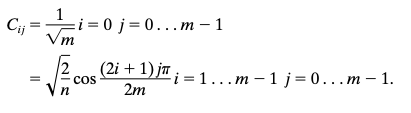
\includegraphics[width=0.75\columnwidth]{lossless_c.png}
  \end{figure}
  \item\textcolor{red}{\textbf{Comment.}} This math format is highly misleading.
  \item\textcolor{red}{\textbf{Comment.}} Throughout all text there is no reference to a DCT definition.
  \item \textbf{Define DCT transform} as $f=CFC^T$.
  \item \textbf{Define inverse DCT transform} as $F=C^TfC$.
  \item\textcolor{red}{\textbf{Comment.}} The notation for $F$ and $f$ is nonstandard.
  \item Finite precision causes quantization of $C$.
  \item\textcolor{red}{\textbf{Comment.}} There are no details or references of how the decimal (not binary!) places are quantized.
  \item If $C$ has $B$ \textbf{decimal places of precision}, $f$ would have $2B$.
  \item $C$ is not unitary, so redefine $F=C^{-1}f(C^T)^{-1}$.
  \item\textcolor{red}{\textbf{Comment.}} There are no mentions to the orthogonality of $C$, necessary to $C^{-1}=C^T$.
  \item $B>1$ otherwise $C^{-1}$ doesn't exist.
  \item\textcolor{red}{\textbf{Comment.}} Because $det(C)=0$ em $B=1$.
  \item $F$ requires about $2m^3$ multiplications and $m-1$ additions.
  \item\textcolor{red}{\textbf{Comment.}} I couldn't verify the number of additions.
  \item Consider the following \textbf{ranking of the coefficients}. Choose to retain only the first $w$, zero out the others.
  \item\textcolor{red}{\textbf{Comment.}} Seams like the RLE method that we saw in class, used in JPEG.
  \begin{figure}[H]
    \centering
    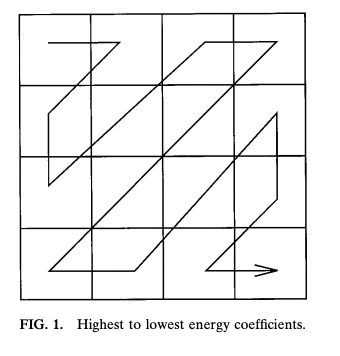
\includegraphics[width=0.50\columnwidth]{lossless_fig1.png}
  \end{figure}
  \item $Fn$ is the $F$ cropped to the first $w$.
  \item \textbf{Residual error} $E=F-Fn$.
  \item $E$ and $Fn$ can reconstruct $F$.
  \item With the first $w$ coefficients, save their \textbf{difference from the respective coefficient form the block on its left}. This decorrelates (removes) the first-order entropy.
  \item\textcolor{red}{\textbf{Comment.}} Why? This is very baffling. The reference [7] should have been mentioned here.
  \item Use an entropy encoder on $E$ like Huffman or arithmetic.
  \item\textcolor{red}{\textbf{Comment.}} References? I don't know the second one.
  \item $B$ has low impact on $E$'s entropy.
  \item Given $m=8$, $B=2$ seams to achieve maximal compression.
  \item There seams to be $w\propto-E$.
  \item However larger $w$ increases $E$ entropy and the overall memory consumption.
  \item\textcolor{red}{\textbf{Comment.}} Why? Could have showed some graphs varying $m$, $B$ and $w$.
  \item \textbf{Potential compression statistic} $p$:
  \begin{figure}[H]
    \centering
    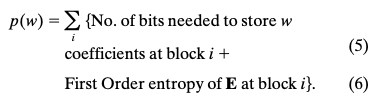
\includegraphics[width=0.75\columnwidth]{lossless_p.png}
  \end{figure}
  \item $p(w)$ has an global minimal as $w$ increases to $m^2$. The value depends on the image and on the scan [6].
  \item The scan form fig.1 is \textbf{optimal if the image data follows a first-order Markov process} [7].
\end{itemize}

\subsubsection*{Experiments}

\begin{itemize}[noitemsep]
  \item Images \textbf{Cameraman}, \textbf{Baboon} and \textbf{Moon}, $256\times256$ gray scale $256$; $m=8$, $w=3$ from $p(w)$, $B=2$; compared to the seven present (1997) JPEG lossless standards.
  \item\textcolor{red}{\textbf{Comment.}} Classical choices, however the pdf versions have unusual artifacts. Though commonly used as test images, they are just too few examples for the sake of comparison. Large datasets with imagens sensitive to loss should have been benchmarked.
  \item Overhead of $3072$, against almost nothing from JPEG.
  \item $E$ and $Fn$ have less entropy than the JPEG preprocessors.
  \item\textcolor{red}{\textbf{Comment.}} The compression ratio for the test images using standard entropy encoder is inconclusive to whether it is better than any of the JPEG standards.
  \item The \textbf{Rice coder} [11, 12] is adaptive and has efficient hardware implementation [12], used to compress $E$.
  \item An adaptive \textbf{Huffman coder} is used for the overhead.
  \item\textcolor{red}{\textbf{Comment.}} The compression ratio for the test images using the Rice and the Huffman coders is still inconclusive. All the methods vary strongly and non-proportionally.
\end{itemize}

\subsubsection*{Conclusion}

\begin{itemize}[noitemsep]
  \item The method performed as average against the JPEG standards, even using a standard entropy coder.
\end{itemize}

\textcolor{red}{\textbf{Final comment.}} Not only the seven JPEG standards are still the principal ones, but also there not newer great advances on general lossless compression after 1997, regarding only the references sited on \href{https://en.wikipedia.org/wiki/Lossless_JPEG}{en.wikipedia.org/wiki/Lossless\_JPEG}. There are no comments about the resources reuired by algorithm, as well as the benchmarking is pretty limited. As the JPEG already offers on average the same compression ratio with a more studied and optimized implementation based roughly on the same core ideas, I couldn't find the advantages of the proposed method.

\end{document}
